\section{Block rewrites, source exposure and resource constraints}\label{sec:rewrites}
\subsection{The rewrite grammar and its threshold}
\begin{definition}[rewrite]\label{def:rewrite}
Let $z\in\ker_{\Z}V_A$ with $z=z^+-z^-$, and let $u$ and $v$ be arrangements of the contents $z^+$ and $z^-$. A \emph{block rewrite} is the replacement $p\cdot u\cdot s\to p\cdot v\cdot s$ of a contiguous block, where $p,s$ are words. Because $R(u)=R(v)$ the state after $p\cdot u$ equals the state after $p\cdot v$, so the suffix $s$ and the endpoint are unchanged. The \emph{rewrite graph} of a source $m$, an endpoint and a move set $M$ of kernel vectors has the admissible histories as vertices and the legal swaps and the legal block rewrites with $z\in\pm M$ as edges; its components are the \emph{rewrite classes}. A rewrite class is a union of swap classes.
\end{definition}
\begin{theorem}[block threshold]\label{thm:block}
Let $p\cdot u\cdot s$ be admissible from $m$. Then $p\cdot v\cdot s$ is admissible from $m$ iff $v$ is admissible from the state $x_p$ reached after $p$, i.e.\ iff $\lcm(K(p u s),K(p v s))\mid m$. The rewrite is thus an event local to the prefix state $x_p$: its executability depends on $x_p$ only through the valuations the block needs.
\end{theorem}
\begin{proof}
The prefix $p$ is common and admissible. After $p\cdot v$ the state is the same as after $p\cdot u$, so the suffix $s$ is admissible from it; the only remaining condition is the admissibility of $v$ from $x_p$. The equivalence with the $\lcm$ is the threshold law applied to the two words.
\end{proof}
\prov{CW-0371}{D4-T3}{PROVED}{FULL}
\emph{Check.} $425$ random cases of the criterion were replayed in this work, with $0$ violations (cited: $11\,000$ randomized tests in the programme's records).

\subsection{Saturation and the quotient description}
\begin{theorem}[saturation]\label{thm:saturation}
Suppose that the contents of the histories from $m$ to a fixed endpoint are connected by moves of a set $M$ (a Graver basis suffices) staying inside the fibre, and that $P(c)\mid m$ for every content $c$. Then the histories form a single rewrite class.
\end{theorem}
\begin{proof}
By \cref{prop:sat} every arrangement of every content is admissible, so each content is one swap class. For a move $z$ taking $c$ to $c'=c+z$, take any history of $c$, swap it into the form $u\cdot r$ with $u$ an arrangement of $z^-$ and $r$ the rest; then $v\cdot r$ is admissible by the same proposition and joins the two swap classes. Connectivity of the fibre under $M$ now gives connectivity of the rewrite graph. (A Graver basis is a Markov basis, \cite{Sturmfels1996,DiaconisSturmfels1998}.)
\end{proof}
\prov{CW-0374}{D4-T6a}{PROVED}{FULL}
\begin{proposition}[quotient description]\label{prop:quotient}
The rewrite classes are exactly the connected components of the graph whose nodes are the swap classes and whose edges are the \emph{exposed redexes}: a redex $u$ or $v$ occurring as a contiguous block in some word of a class whose replacement is admissible.
\end{proposition}
\begin{proof}
By \cref{def:rewrite}: a rewrite edge between two histories is by definition an exposed redex, and the classes of the graph with swap edges and rewrite edges are the components of the quotient by swap classes.
\end{proof}
\prov{CW-0375}{D4-T6b}{PROVED}{FULL}
\begin{corollary}[three obstruction types]\label{cor:trichotomy}
Below the saturation condition a rewrite graph can be disconnected for three separately observable reasons: (a) \emph{algebraic}, the content fibre is disconnected under $M$; (b) \emph{exposure}, contents are linked by a move of $M$ but no history has a contiguous redex because the context labels cannot be moved out of the block; (c) \emph{emptiness}, some content has no admissible history from $m$.
\end{corollary}
Algebraic obstructions hold at every source and are the subject of \cref{prop:graver}; exposure and emptiness are source-dependent and are separated for a test family below.

\subsection{Positive and negative completeness}
\begin{proposition}[three labels; finite-exact]\label{prop:T6c}
For the alphabet $\{1,2,3\}$, swaps together with the single move $1^7\leftrightarrow2^23^4$ connect all histories of equal source and endpoint, in the box $v_2(m)\le1$, $v_3(m)\le4$, $c_3\le8$ with fibre length $\ge2$ ($30$ fibres, $840$ fibre-source pairs, no disconnected pair; $16$ fibres and $364$ pairs re-checked independently in the programme). General $m$ is open: the fibres are the rank-one chains $c+t(7,-2,-4)$, so a proof would need an exposed redex for every consecutive pair of contents. \stat{finite-exact}.
\end{proposition}
\prov{CW-0376}{D4-T6c}{FINITE-EXACT}{FINITE}
\begin{proposition}[the Graver basis cannot be omitted]\label{prop:graver}
On the alphabet $\{1,2,3,8\}$ let $z_1=(1,-4,0,2)$ and $z_2=(7,-2,-4,0)$. The fibre $\{3^28,\ 1^32\}$ at endpoint $288=R(3)^2R(8)=R(1)^3R(2)$ contains two contents that are \emph{not} joined by $\pm z_1,\pm z_2$ and swaps: neither content admits a move (the contents $(0,0,2,1)$ and $(3,1,0,0)$ have $c_2\le1$, $c_3\le2$, $c_1\le3$, so none of $c\pm z_1$, $c\pm z_2$ is nonnegative). They are joined by the Graver vector $z_3=(3,1,-2,-1)=\bigl((3,1,0,0)-(0,0,2,1)\bigr)$. \stat{proved} for the explicit pair; the programme's census finds $498$ of $816$ fibres deficient for $\{z_1,z_2\}$ \stat{finite-exact}, not re-run here.
\end{proposition}
\prov{CW-0379}{D4-T7c}{PROVED}{FULL}
So generating the kernel is not enough: the move set must contain a Graver (Markov) basis for the fibre to be algebraically connected.

\subsection{An exposure dichotomy for all \texorpdfstring{$j$}{j}}
For $j\ge1$ consider the family $U_j=\{2^4,3^j\}$, $V_j=\{1,8^2,3^j\}$ with the move $2222\leftrightarrow$ any arrangement of $\{1,8,8\}$ (the kernel vector $z_1$); $R(2)^4=R(1)R(8)^2=3^8/2^4$. Write $a=v_2(m)$, $b=v_3(m)$.
\begin{theorem}[exposure dichotomy]\label{thm:Fj}
For every $j\ge1$: both contents have admissible histories from $m$ iff $b+8\ge j$ and $(a,b)\ne(0,0)$. In that case the swap-and-rewrite space is connected iff $b\ge1$ or $a\ge4$ (i.e.\ iff $3\mid m$ or $16\mid m$), and otherwise it has exactly two components, one swap class per content.
\end{theorem}
\begin{proof}
\emph{Realisability.} Each $2$ adds $2$ to $v_3$, each $8$ adds $4$, and each $3$ removes $1$, so the final $v_3$ is $b+8-j\ge0$. If $a=b=0$, then $U_j$ cannot start ($2$ needs $v_2\ge1$ and $3$ needs $v_3\ge1$) and $V_j$ stalls after the leading $1$ ($8$ needs $v_2\ge3$, $3$ needs $v_3\ge1$; a leading $1$ gives $v_2=2$ only). Otherwise explicit words exist: for $b\ge1$, $3,2,2,2,2,3^{j-1}$ and $3,1,8,8,3^{j-1}$; for $b=0,a\ge1$ (so $j\le8$), $2,3,2,2,2,3^{j-1}$ and $1,8,3,8,3^{j-1}$.

\emph{One swap class per content.} Let $A,B$ be coprime labels such that $2v_p(A+1)\ge v_p(B)$ for $p\mid B$ and $2v_q(B+1)\ge v_q(A)$ for $q\mid A$ (here $(2,3)$ and $(8,3)$: $2v_3(3)=2\ge1$, $2v_2(4)=4\ge1$, $2v_3(9)=4\ge1$). Claim: from any state, all admissible orderings of a multiset $\{A^s,B^t\}$ lie in one swap class. Induct on the length. Take admissible $A\cdot r$ and $B\cdot r'$. In $A\cdot r$ the first $B$ occurs after some $A$'s; it can be moved to the front of $r$ by legal adjacent swaps: at the state after the first $A$ we have $v_p\ge 2v_p(A+1)\ge v_p(B)$ for $p\mid B$, so $B$ is legal there; the $A$'s it passes only gain resources, since $\Delta_q(B)=2v_q(B+1)\ge0$ for $q\mid A$ and $q\nmid B$. Thus $A\cdot r$ is in the class of $A\cdot B\cdot r''$. Symmetrically $B\cdot r'$ is in the class of $B\cdot A\cdot r'''$. Both orders $AB$ and $BA$ are legal from the start state (each letter is legal at the start by assumption, and the other raises the resources of the first), with the same state afterwards; by induction the arrangements after them lie in one class, so the two classes coincide. For $V_j$ the label $1$ can be moved to the front by legal swaps (it divides everything and only raises $v_2$), so the claim applies after it.

\emph{Connectivity.} If $b\ge1$, both $3\cdot2222\cdot3^{j-1}$ and $3\cdot(1,8,8)\cdot3^{j-1}$ are admissible: after the leading $3$ the valuation $v_2\ge4$, the blocks leave $v_3=b+7\ge j-1$, and for $(1,8,8)$ the walk of $v_2$ is $\ge6,\ge3,\ge0$. They have one endpoint, so the block rewrite joins the two swap classes. If $a\ge4$, $b=0$ (so $j\le8$), then $2222\cdot3^j$ and $1\cdot8\cdot8\cdot3^j$ are admissible and the same argument applies.

\emph{Obstruction ($3\nmid m$, $a\le3$, $(a,b)\ne(0,0)$).} A label $3$ is applicable only after $v_3$ has been raised by a $2$ or an $8$. In $U_j$ all $2$s lie in the redex $2222$, in $V_j$ all $8$s lie in the redex (an arrangement of $\{1,8,8\}$). So no $3$ precedes a redex, the redex starts at position $0$ with $v_2=a\le3$, and: $2222$ needs $v_2\ge4$; the arrangements $(1,8,8)$, $(8,1,8)$ need $a\ge4$, $(8,8,1)$ needs $a\ge6$. No redex is ever exposed, so the two swap classes are not joined.
\end{proof}
\prov{CW-0391}{B-T9}{PROVED}{FULL}
\begin{figure}[tbp]\centering
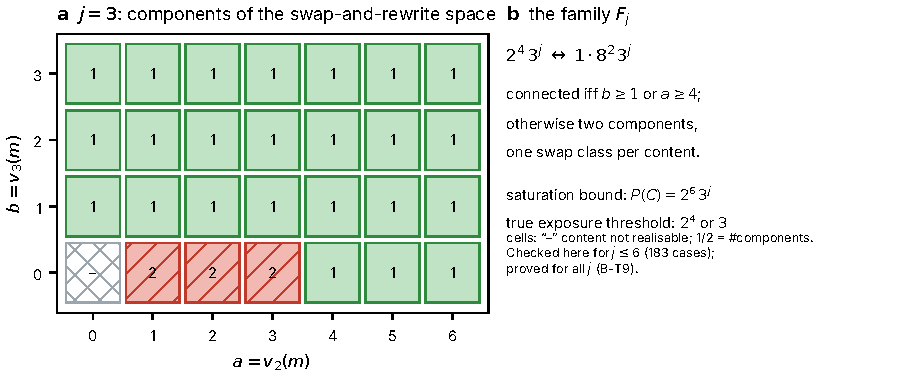
\includegraphics[width=0.78\linewidth]{fig18_rewrite_exposure}
\caption{\textbf{Components of the swap-and-rewrite space of $2^43^j\leftrightarrow1\cdot8^23^j$ for $j=3$ (finite-exact table, matching \cref{thm:Fj}).} The entry at $(a,b)=(v_2(m),v_3(m))$ is the number of components: $0$ (nothing realisable) at $(0,0)$, $2$ at $b=0$ and $a\in\{1,2,3\}$ (exposure obstruction), $1$ elsewhere. Colour is redundant with the printed integers. Theorem illustrated: \cref{thm:Fj}.}\label{fig:exposure}
\end{figure}
\noindent The figure above is \cref{fig:exposure}; its caption states the exactness of what is drawn.
\begin{remark}[supersession and sharpness]\label{rem:supersede}
The source release D4-T7b stated the dichotomy for $j\le8$ (finite-exact) and marked general $j$ open; the addendum proves it for all $j$ (the sufficient direction above, and the realisability bound $j\le b+8$, are what made the finite range natural). The saturation bound of \cref{thm:saturation} for this family is $2^63^j$ ($P(U_j)=2^43^j$, $P(V_j)=2^63^j$) while the true connectivity boundary is $3\mid m$ or $16\mid m$: the product bound is not sharp, and the sharp boundary is an exposure condition, not an all-arrangements condition.
\end{remark}
\prov{CW-0377}{D4-T7a}{PROVED}{FULL}
\prov{CW-0378}{D4-T7b}{MIXED}{SPLIT}
We recomputed the dichotomy for $j\le6$ over all $(a,b)$ with $a\le6$, $b\le j$ in this work, and it agrees ($183$ rows, no violation).

\subsection{Content-changing rewrites can create loops}
\begin{example}[the join example; exact]\label{ex:join}
$R(2)R(8)R(63)=R(5)R(9)R(35)=20736/7$. At the sources $m=280$ and $m=840$ the four histories $(2,63,8)$, $(8,63,2)$, $(5,9,35)$, $(35,9,5)$ have pairwise different traces; there is no legal swap, so the swap space is $4$ points with $4$ swap classes. The block replacements $(2,63,8)\leftrightarrow(5,9,35)$, $(2,63,8)\leftrightarrow(35,9,5)$, $(8,63,2)\leftrightarrow(5,9,35)$, $(8,63,2)\leftrightarrow(35,9,5)$ are all admissible and form a $4$-cycle: one rewrite class, cells $\{0:4,1:4\}$, $\mathbb F_2$-Betti vector $(1,1)$. A content-changing relation creates a loop out of a disconnected swap space.
\end{example}
\prov{CW-0380}{D4-T8a}{PROVED}{FULL}
\begin{problem}[open: homotopy type of extended complexes]\label{prob:extended}
The extended complex of histories with swaps and block rewrites has no coherence cells: braid hexagons and relations between overlapping moves are not filled, so its Betti numbers are invariants of this specific complex only. Its homotopy type, the effect of adding coherence cells, and Künneth-type behaviour for products of loop sides are open. A cycle in a restricted complex need not be a cycle in the complete one. \stat{open}.
\end{problem}
\prov{CW-0381}{D4-T8b}{OPEN}{OPEN}
